\documentclass{beamer}

\mode<presentation> {
	\usetheme{CambridgeUS}
	\usecolortheme{crane}
	\usefonttheme{default}
}

\usepackage{graphicx}
\usepackage{booktabs}
\usepackage{ragged2e}
\usepackage[export]{adjustbox}
\usepackage{minted}
\usemintedstyle{monokai}

\usepackage{aut}

%----------------------------------------------------------------------------------------
%	TITLE PAGE
%----------------------------------------------------------------------------------------
\title[CoAP middle server for IoT platform]{Roadmap of IoT Platforms}
\author{IoT Lab @ AUT}
\institute[] {
  Amirkabir University of Technology
}
\date{\today}
\titlegraphic{\hspace*{5cm}
\includegraphics[width=2cm]{figs/aut_logo.jpeg}}

\begin{document}

\begin{frame}
\titlepage
\end{frame}

%----------------------------------------------------------------------------------------
%	PRESENTATION SLIDES
%----------------------------------------------------------------------------------------

%------------------------------------------------
\begin{frame}
	\frametitle{Outline}
	\vspace{.1cm}
	\begin{itemize}
		\justifying
		\item Architecture
		\item<2-> Simple IoT Management Protocol
		\item<3-> Roadmap
	\end{itemize}
\end{frame}

%------------------------------------------------
\begin{frame}
	\frametitle{Outline}
	\vspace{.1cm}
	\begin{itemize}
		\justifying
		\item Architecture
		\item \textcolor{LightGray}{Simple IoT Management Protocol}
		\item \textcolor{LightGray}{Roadmap}
	\end{itemize}
\end{frame}

%------------------------------------------------
\begin{frame}
	\frametitle{Architecture}
	\vspace{.1cm}
	\hspace*{.75cm} 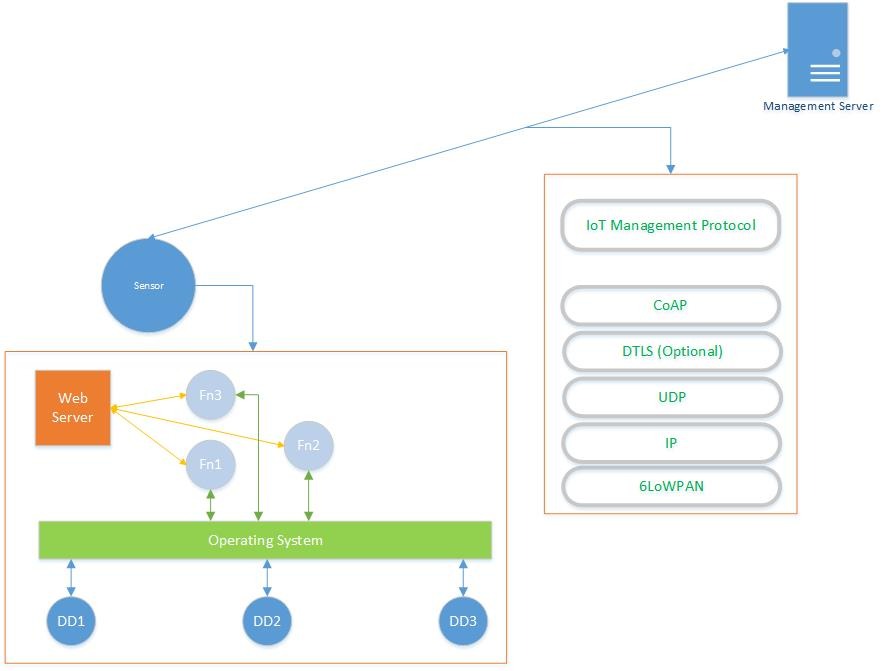
\includegraphics[width=10.5cm]{../architecture/architecture.jpg}
\end{frame}

%------------------------------------------------
\begin{frame}
	\frametitle{Outline}
	\vspace{.1cm}
	\begin{itemize}
		\justifying
		\item \textcolor{LightGray}{Architecture}
		\item Simple IoT Management Protocol
		\item \textcolor{LightGray}{Roadmap}
	\end{itemize}
\end{frame}

%------------------------------------------------
\begin{frame}[fragile]
	\frametitle{Simple IoT Management Protocol}
	\begin{minted}
		[
			frame=lines,
			obeytabs,
			showtabs,
			tabsize=4,
			baselinestretch=1.2,
			fontsize=\footnotesize,
			bgcolor=LightGray,
		]{json}
{
	"id": 1,
	"type": "light",
	"variables": [
		{
			"name": "light_intensity",
			"type": "int",
			"permission": "wr"
		},
	\end{minted}
\end{frame}

%------------------------------------------------
\begin{frame}[fragile]
	\frametitle{Simple IoT Management Protocol}
	\begin{minted}
		[
			frame=lines,
			obeytabs,
			showtabs,
			tabsize=4,
			baselinestretch=1.2,
			fontsize=\footnotesize,
			bgcolor=LightGray,
		]{json}
		{
			"name": "reset",
			"type": "func",
			"parameters": [
				{
					"name": "interval",
					"type": "int"
				}
			],
			"retrun": "void"
		}
	]
}
	\end{minted}
\end{frame}

%------------------------------------------------
\begin{frame}
	\frametitle{Outline}
	\vspace{.1cm}
	\begin{itemize}
		\justifying
		\item \textcolor{LightGray}{Architecture}
		\item \textcolor{LightGray}{Simple IoT Management Protocol}
		\item Roadmap
	\end{itemize}
\end{frame}

%------------------------------------------------
\begin{frame}
	\frametitle{Roadmap}
	\begin{itemize}
		\item Complete SIMP Definition
		\item Complete SIMP Tools
		\item Implement Protocol Stack on Node
		\item Implement WebServer On Node
		\item Impelemnt Management Server
	\end{itemize}
\end{frame}



\end{document}
